\section{Desafio}

O desafio do subsistema de Rastreio, Telemetria e Comando (TT\&C) é exemplificado na figura~\ref{fig:challenge}.

\begin{figure}[H]
    \centering
    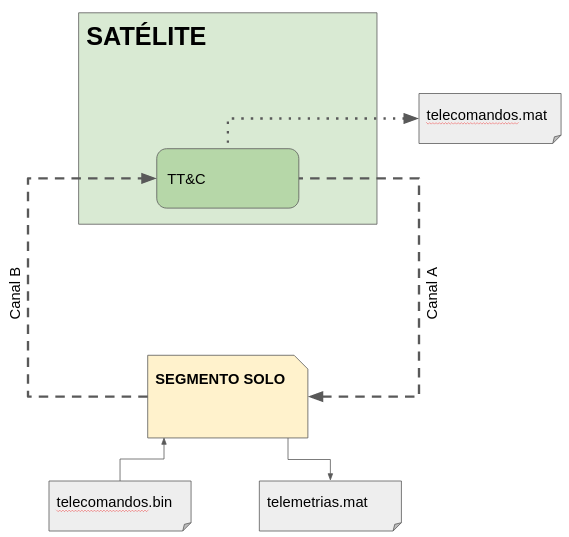
\includegraphics[width=0.75\textwidth]{figures/ttec.png}
    \caption{Diagrama de blocos do desafio do subsistema de TT\&C}
    \label{fig:challenge}
\end{figure}

Em suma, o desafio busca prover evidência de que o subsistema citado é capaz de receber telecomandos através do Canal B, decodificar os \textit{Space Packets}, identificar os \textit{Data Packets} e separar a informação recebida.
Identificar a informação a ser transmitida em \textit{Data Packets}, codificar os \textit{Space Packets} a serem enviados, modular o sinal para ser enviado via canal A.

Para isso será fornecido um modelo em MatLab/Simulink, da MathWorks, de forma simular o Segmento Solo.

O teste de telecomandos do desafio consta de:

\begin{enumerate}[label=(\roman*)]
    \item Receber um sinal modulado de telecomando pelo canal B \textbf{RQ-SYS-211,RQ-SYS-213}
    \item Demodular o sinal \textbf{RQ-TTC-232}
    \item Separar o \textit{Space Packet} em Cabeçalho e \textit{Data Packet} \textbf{RQ-TTC-312}
    \item Separar e Decodificar  cada um dos campos do Cabeçalho AX.42 \textbf{RQ-TTC-322}
    \item Separar e Decodificar cada um dos campos do \textit{Data Packet} \textbf{RQ-TTC-322}
    \item Verificar a validade do \textit{frame} de Telecomando segundo heurística \textbf{RQ-TTC-421}
\end{enumerate}

A fim de gerar evidências do cumprimento destes requisitos, a critério de desafio, deverá ser salvo um arquivo MatLab \textit{Workspace} (.mat) configurado da forma com na tabela~\ref{tab:telecomandos.mat}

\begin{table}[H]
    \centering
    \resizebox{0.85\linewidth}{!}{%
    \begin{tabular}{l|l|l|l}
        Variável & Tipo & Tamanho & Valor\\ \hline
        raw\_data & double array & $n \times 1$ & N/A \\
        space\_packet & double array & $n \times 2$ & [ax42\_header data\_packet] \\
        ax42\_header & double array & $n \times 4$ & [flag address control pid] \\
        address & char array & $n \times 4$ & [fonte fonte\_ssid destino destino\_ssid] \\
        data\_packet & double array & $n \times 4$ & [code subcode length\_telecomando telecomando] \\
        telecomando & double array & $n \times 2$ & [tc\_parameter fcs] \\ \hline
    \end{tabular}
    }
    \caption{Definição do arquivo \textit{MatLab Workspace}}
    \label{tab:telecomandos.mat}
\end{table}

Onde $n$ é o número de telecomando recebidos e demodulados.

O item a seguir define o requisito associado ao envio do arquivo \textit{MatLab Workspace}.

\begin{table}[H]
    \centering
    \begin{tabular}{|c|p{0.7\textwidth}|}
        \hline
        \rowcolor{orange}
        \textbf{RQ-TTC-501} & \textbf{O arquivo MatLab \textit{Workspace} deve ser entregue à comissão organizadora junto com o modelo do TT\&C do desafio.} \\ \hline
    \end{tabular}
    \label{tab:rq-ttc-501}
\end{table}

O teste de telemetrias consta de:

\begin{enumerate}[label=(\roman*)]
    \item Codificar o \textit{Data Packet} \textbf{RQ-TTC-331}
    \item Codificar o \textit{Space Packet} \textbf{RQ-TTC-311}
    \item Modular a mensagem em BPSK \textbf{RQ-TTC-231}
    \item Transmitir o sinal modulado via canal A \textbf{RQ-SYS-212} \textbf{RQ-SYS-211}
\end{enumerate}

O comissão organizadora utilizará de um \textit{script} MatLab para a leitura das telemetrias e geração do \textit{MatLab Workspace} \verb|telemetrias.mat| a fim de validar os requisitos realcionados. 

\subsection{Critérios de Pontuação e Classificação}

O critério de pontuação das equipes devem seguir a tabela~\ref{tab:classificacao}.

% Please add the following required packages to your document preamble:
% \usepackage{graphicx}
\begin{table}[H]
% \resizebox{0.65\linewidth}{!}{%
\centering
\begin{tabular}{c|c}
\hline
\multicolumn{1}{c|}{\textbf{Item}}        & \textbf{Peso} \\ \hline
\textit{Envio do Modelo Simulink do TTeC} & 1             \\
\textit{RQ-SYS-211}                       & 1          \\
\textit{RQ-SYS-212}                       & 1          \\
\textit{RQ-SYS-213}                       & 1          \\
\textit{RQ-TTC-231}                       & 1          \\
\textit{RQ-TTC-232}                       & 1          \\
\textit{RQ-TTC-311}                       & 1          \\
\textit{RQ-TTC-312}                       & 1          \\
\textit{RQ-TTC-321}                       & 1          \\
\textit{RQ-TTC-322}                       & 1          \\
\textit{RQ-TTC-323}                       & 1          \\
\textit{RQ-TTC-331}                       & 1          \\
\textit{RQ-TTC-332}                       & 1          \\
\textit{RQ-TTC-421}                       & 1          \\
\textit{RQ-TTC-501}                       & 1          \\ \hline
\end{tabular}%
% }
\caption{Pontuação do Desafio}
\label{tab:classificacao}
\end{table}

A nota de cada equipe será calculada da seguinte forma:

\begin{equation}
    NOTA=\left (\frac{[\textrm{Entrega do Modelo}] + \frac{\sum_{i=0}^{15}[\textrm{RQ-TTC}]_i}{15}}{2} \right ) \times 100
\end{equation}

As notas de cada equipe variarão entre 0 e 100.

Os critérios de desempate no caso de duas ou mais equipes terminarem com a mesma pontuação seguem a ordem a seguir:

\begin{enumerate}[label=(\roman*)]
    \item Menor número de blocos presentes no modelo simulink do TT\&C;
    \item Menor número de linhas de código, caso utilizado, desconsiderando-se comentários;
    \item Horário de envio dos arquivos requeridos da equipe à comissão organizadora, horário local (GMT-3 Brasília).
\end{enumerate}